\subsection{Definition (2-D)}

The aim of this example is to simulate the stationary groundwater flow in an isotropic and heterogeneous porous medium. In order to consider the heterogeneous of hydraulic conductivity, a 2-D numerical model is built. The heterogeneous distribution of hydraulic conductivity is shown in Fig. \ref{KDis}. The aquifer is assumed isotropic, heterogeneous, saturated and stationary.

\begin{figure}[htb]
\centering
\vspace{-10pt}
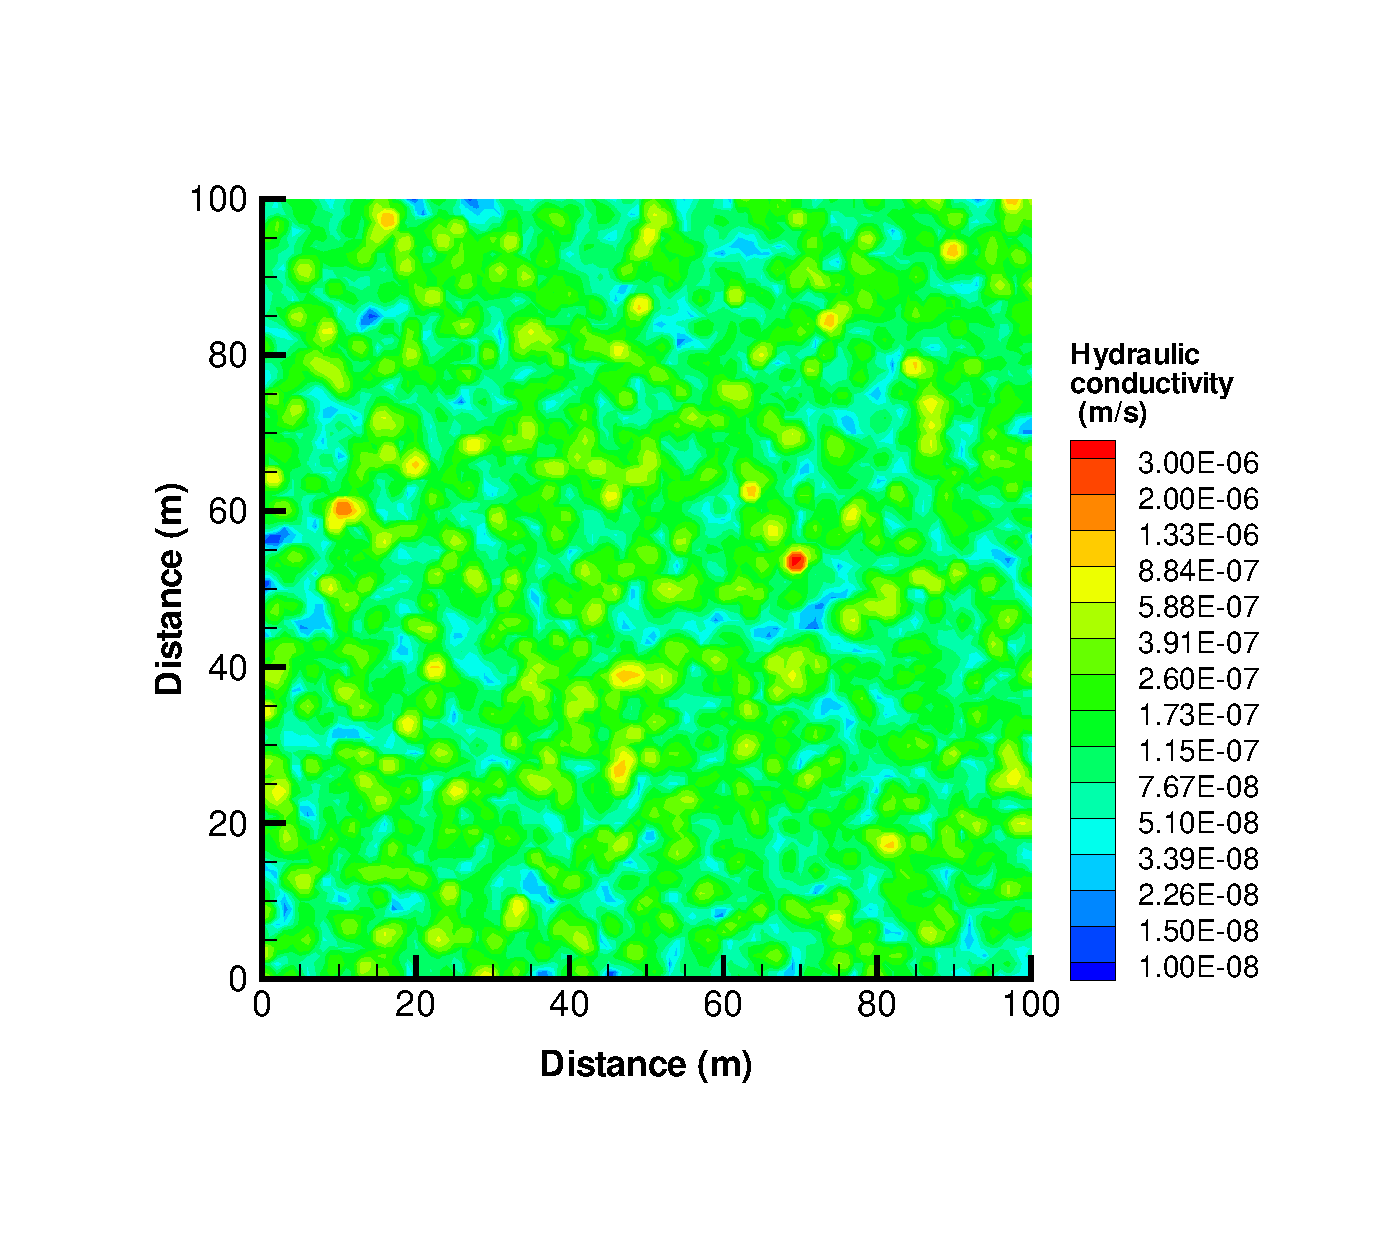
\includegraphics[width=0.8\textwidth]{Chapter5/figure/KDis.eps}
\vspace{-10pt}
\caption{Calculation model~(2-D): hetergeneous hydraulic conductivity distribution.}
\vspace{-10pt}
\label{KDis}
\end{figure}

For the two-dimensional simulation, the cube consisting of a porous medium is simplified as a square with an area of 10000~m$^2$. The calculation model includes 10000 quad elements and 10201 nodes. At the left boundary  a constant head of 10~m and the right boundary  a constant head of 9~m are specified in order to create a pressure gradient. 

\subsection{Results (2-D)}

As shown in figure \ref{HeadDis}, the head distribution of the groundwater flow in a heterogeneous medium is depicted complying with the distribution of the hydraulic conductivity. 

\begin{figure}[htb]
\centering
\vspace{-10pt}
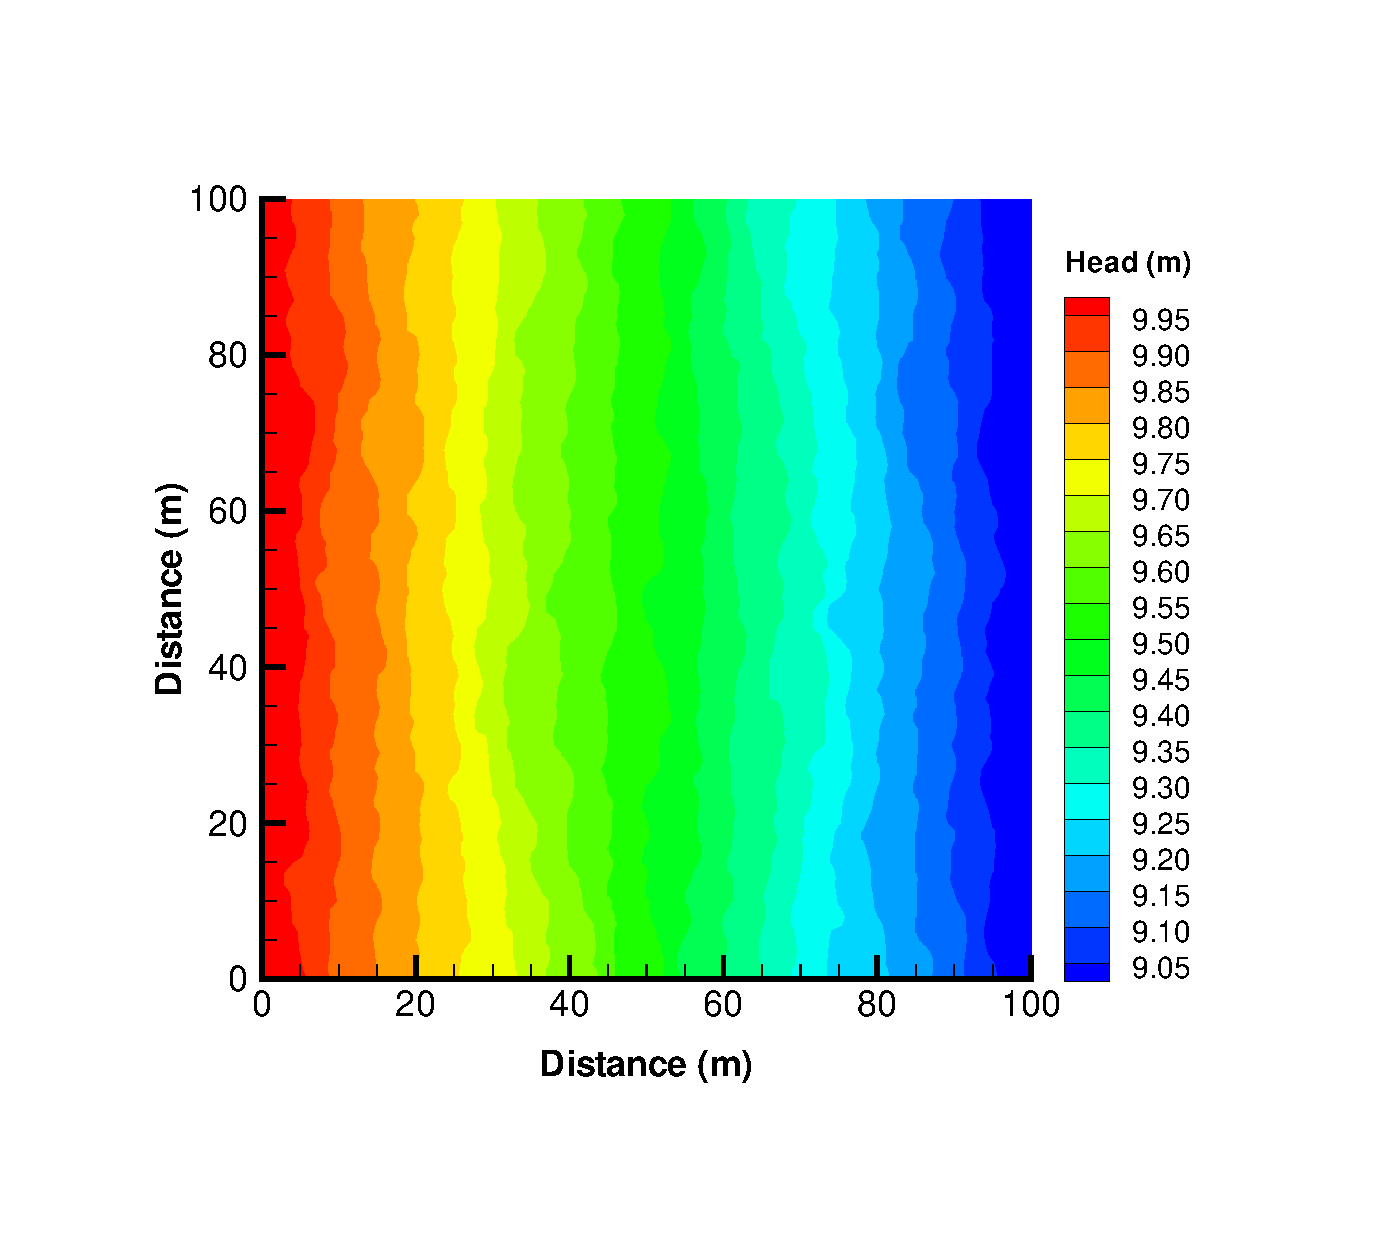
\includegraphics[width=0.8\textwidth]{Chapter5/figure/HeadDis.eps}
\vspace{-10pt}
\caption{Head distribution in response to isotropic and heterogeneous medium.}
\label{HeadDis}
\end{figure}

\subsection{Definition (3-D)}

For the three-dimensional simulation, the aquifer is defined as a 100~m$\times$ 100~m$\times$ 50~m cuboid. The calculation model includes 60025 hex elements and 65000 nodes.  A constant head of 10~m at the left surface and a constant head of 9~m at the right surface are specified in order to create a pressure gradient. The heterogeneous distribution of hydraulic conductivity is shown in Fig. \ref{KDis3d}.

\newpage

\begin{figure}[htb]
\centering
\vspace{-40pt}
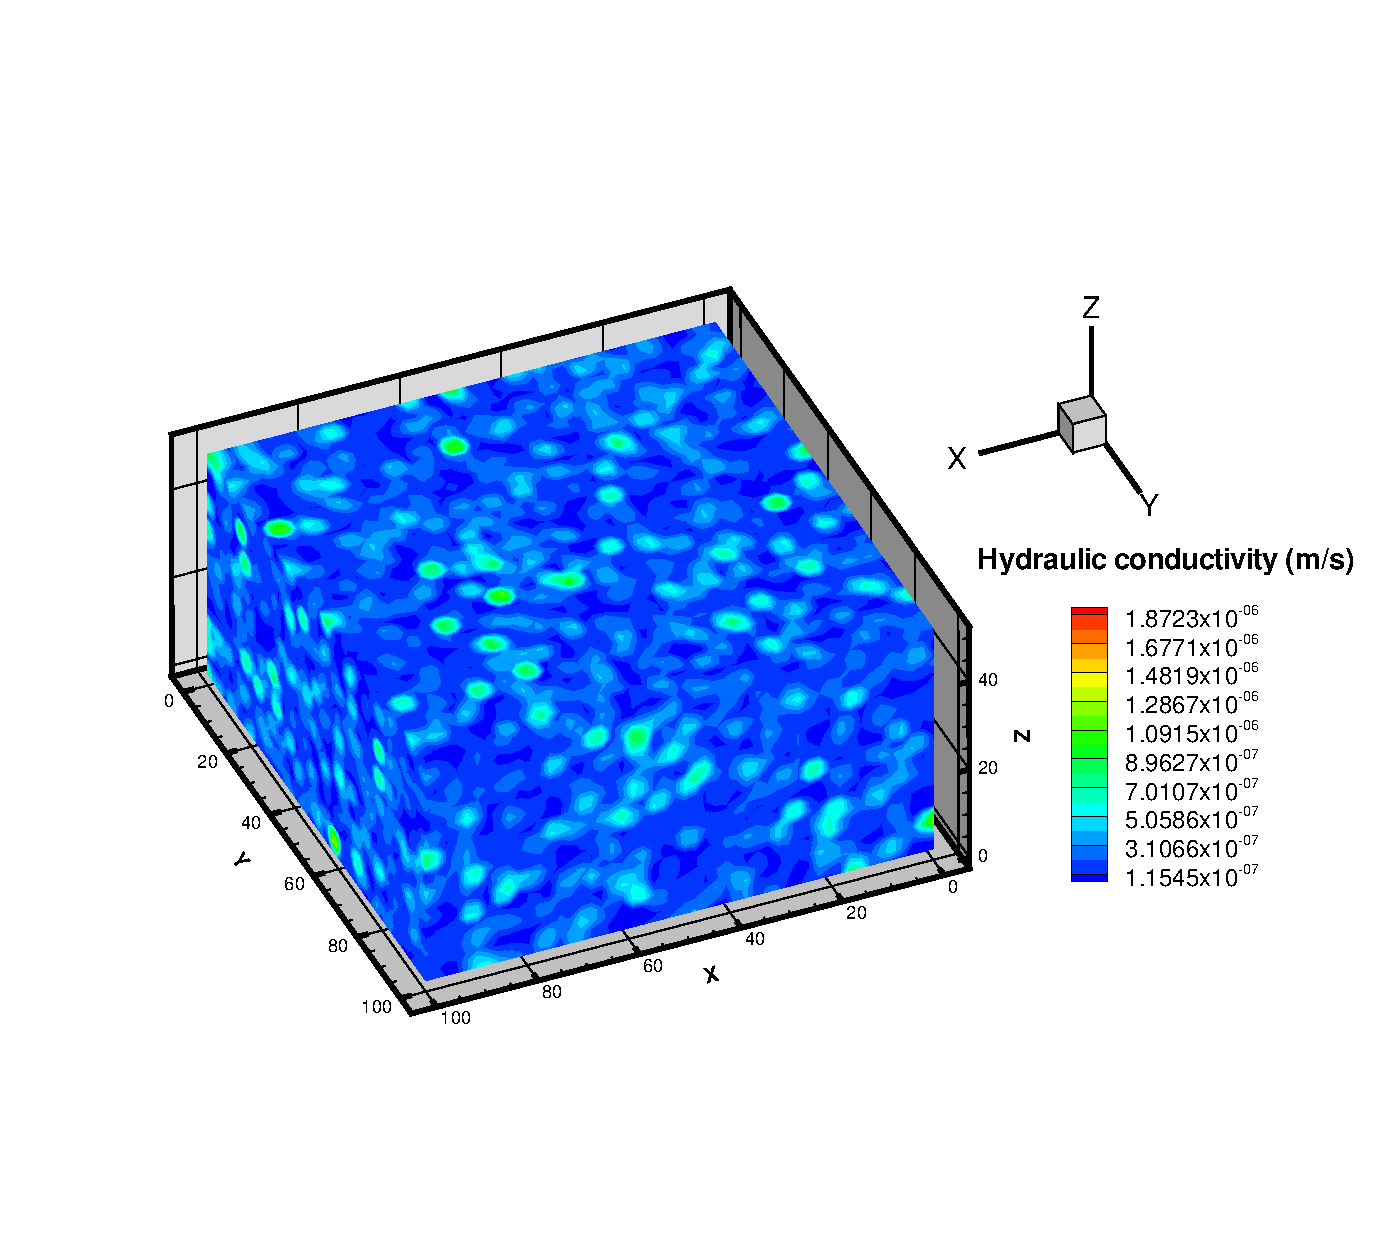
\includegraphics[width=0.8\textwidth]{Chapter5/figure/3DHGWH.eps}
\vspace{-20pt}
\caption{Calculation model~(3-D): hetergeneous hydraulic conductivity distribution.}
\vspace{-10pt}
\label{KDis3d}
\end{figure}

\begin{figure}[htb]
\centering
\vspace{-40pt}
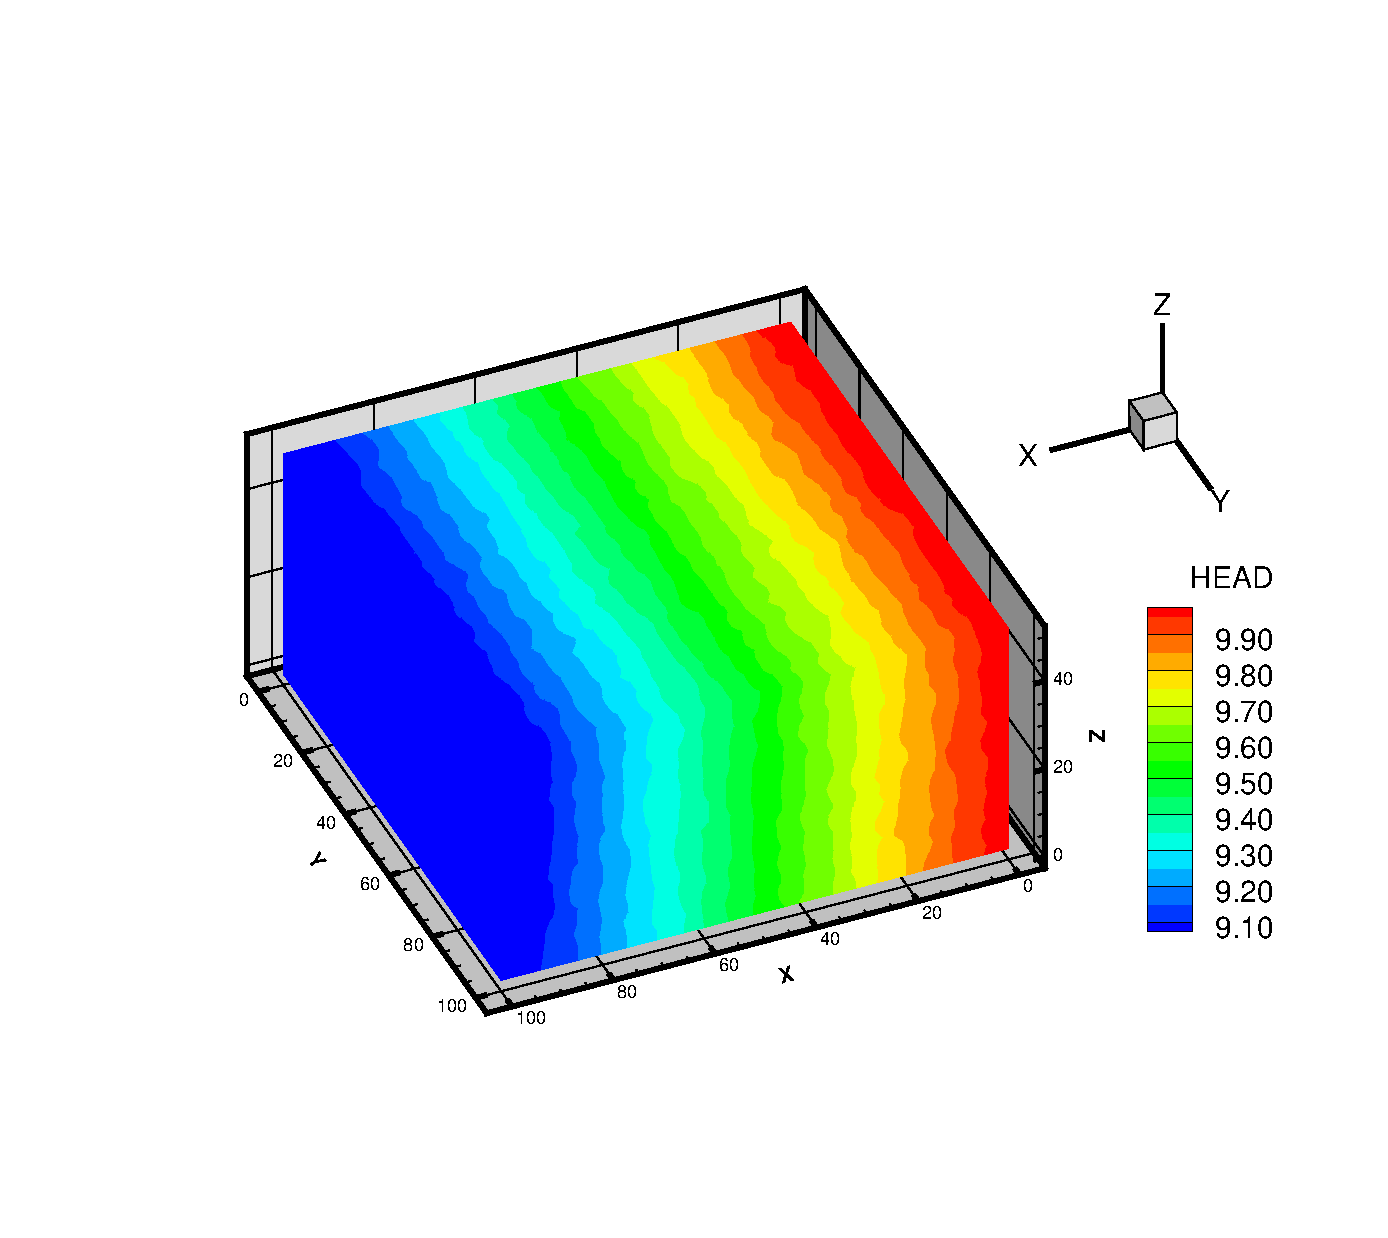
\includegraphics[width=0.8\textwidth]{Chapter5/figure/3DHGWR.eps}
\vspace{-20pt}
\caption{Head distribution in response to isotropic and heterogeneous medium (3-D).}
\vspace{-10pt}
\label{HeadDis3d}
\end{figure}

\subsection{Results (3-D) }

As shown in figure \ref{HeadDis3d}, the 3-D head distribution of the groundwater flow in a heterogeneous medium is depicted in response to the distribution of the hydraulic conductivity. 
